% ----------------------------------------------------------
% Anexos
% ----------------------------------------------------------

% ---
% Inicia os anexos
% ---
\begin{anexosenv}

% Imprime uma página indicando o início dos anexos
\partanexos


\chapter{Tabela de dados}

Para o caso do Loan Club, nem todas as variáveis foram utilizadas. Isto se deve ao fato de que algumas das variáveis em questão são categóricas, outras que representam alguma descrição. Tratam-se de campos que provem informações substanciais mais que para o escopo deste trabalho foram desconsideradas. No caso de variáveis categóricas, seria possível uma conversão para variáveis dummies, mas que para o caso do k médias não devem ser consideradas. Já para os campos que possuem uma informação textual, existem algoritmos que podem fazer análises do conteúdo como \"word to vec\" ou \"bag of words\".

 \label{tab:daypack}
    \begin{tabularx}{\textwidth}{p{.3\textwidth}X}
    \caption{Tabela de campos utilizados para a analise do banco de dados Loan Club}\\
    \toprule
    \textbf{Coluna} & \textbf{Descrição} \\[6pt]
    \midrule
    \endhead

funded\textunderscore amnt & Total do montante comprometido para aquele empr\'estimo at\'e este momento\\
funded\textunderscore amnt\textunderscore inv & Total do montante comprometido pelos investidores para aquele empr\'estimo at\'e este momento\\
grade & Nota atribu\'ida pelo Loan Club\\
loan\textunderscore amnt & A quantia do empr\'estimo do mutu\'ario, podendo ter eventualmente descontos pelo departamento de cr\'edito\\
term & Quantidade de pagamentos do empr\'estimos que pode ser de 36 ou 60 meses\\
int\textunderscore rate & Taxa de juros do empr\'estimo\\
installment & Pagamento devido pelo tomador de empr\'estimo\\
annual\textunderscore inc & Renda anual relatada pelo devedor durante o cadastro\\
dti\textunderscore joint & A raz\~ao entre a quantia total de d\'ividas paga pelos co-mutu\'arios (desconsiderando hipotecas e o empr\'estimo feito pelo Loan Club) dividido pela renda mensal dos co-mutu\'arios\\
delinq\textunderscore 2yrs & Incid\^encias de inadimpl\^encia (eventos ocorridos dentro de 30 dias) dentro de um per\'iodo de 2 anos\\
inq\textunderscore last\textunderscore 6mths & Quantidade de pedidos de empr\'estimos (excluindo carros e hipotecas)\\
open\textunderscore acc & N\'umero de linhas de cr\'editos abertas para o mutu\'ario\\
pub\textunderscore rec & N\'umero de \"derogatory public records\" (trata-se de um registro que pode ser considerado negativo para o mutu\'ario pois indica um risco e denegrindo sua reputa\c c\~ao e dificultando a possibilidade de aquisi\c c\~ao de outros produtos. Entre os valores, \'e poss\'ivel W e F\\
revol\textunderscore bal & Total de cr\'edito que n\~ao foi pago\\
total\textunderscore acc & N\'umero toral de linhas de cr\'editos usada pelo mutu\'ario\\
out\textunderscore prncp & Saldo devedor\\
out\textunderscore prncp\textunderscore inv & Saldo devedor sobre a por\c c\~ao de capital financiado por investidores\\
total\textunderscore pymnt & Pagamentos recebidos at\'e o momento presente sobre o valor financiado\\
total\textunderscore pymnt\textunderscore inv & Pagamentos recebidos at\'e o momento presente sobre o valor financiado pelo investidor\\
total\textunderscore rec\textunderscore int & Juros recebido at\'e a data presente\\
total\textunderscore rec\textunderscore late\textunderscore fee & Taxas de atraso recebido at\'e a presente data\\
total\textunderscore rec\textunderscore prncp & Capital financiado recebido at\'e a data presente\\
collection\textunderscore recovery\textunderscore fee & valor de imposto recuperado de \"charge off\" (declara\c c\~ao de n\~ao quita\c c\~ao de uma d\'ivida)\\
last\textunderscore pymnt\textunderscore amnt & Valor total de pagamento recebido\\
recoveries & valor bruto recuperado de \"charge off\" verificados \\
\bottomrule

\end{tabularx}


 \label{tab:daypack}
    \begin{tabularx}{\textwidth}{p{.3\textwidth}X}
    \caption{Tabela de campos disponíveis em Loan Club e que n\~ao foram utilizados}\\
    \toprule
    \textbf{Coluna} & \textbf{Descrição} \\[6pt]
    \midrule
    \endhead

addr\textunderscore state & Estado de moradia do mutu\'ario\\
annual\textunderscore inc\textunderscore joint & Valor declarado no momento do cadastro da renda anual do co-mutu\'arios (um emprestimo eh realizado com co-mutuarios quando mais de uma pessao eh sao financiadas)\\
application\textunderscore type & Indica se o empr\'estimo ser\'a individual ou se ser\'a feito por mais de uma pessoa (co-mutu\'arios) \\
earliest\textunderscore cr\textunderscore line & M\^es mais recente em que o mutu\'ario abriu uma linha de cr\'edito\\
emp\textunderscore length & Per\'iodo em que o devedor est\'a empregado no trabalho atual, na qual 0 representa menos de 1 ano e 10 pode ser de 10 a mais anos \\
emp\textunderscore title & Descri\c c\~ao breve do emprego do devedor\\
fico\textunderscore range\textunderscore high & Limite superior do score proveniente do FICO a qual o devedor est\'a enquadrado\\
fico\textunderscore range\textunderscore low & Limite inferior do score proveniente do FICO a qual o devedor est\'a enquadrado\\
home\textunderscore ownership & Indica o status do tipo de moradia do tomador de empr\'estimo RENT (aluguel), OWN (casa pr\'opria), MORTGAGE (hipoteca), OTHER (outros)\\
id & vari\'avel de identifica\c c\~ao de cada cliente da Loan Club\\
initial\textunderscore list\textunderscore status & Status inicial e interno da Loans Club do mutu\'ario. Varia entre W e F\\
is\textunderscore inc\textunderscore v & Indica se a renda foi verificada pela Loan Club ou n\~ao ou se a fonte de renda foi verificada\\
issue\textunderscore d & M\^es no qual o empr\'estimo foi financiado\\
last\textunderscore credit\textunderscore pull\textunderscore d & O m\^es mais recente desde que o mutu\'ario adquiriu cr\'edito no financiamento\\
last\textunderscore fico\textunderscore range\textunderscore high & O limite superior do \'ultimo score do FICO em que o mutu\'ario foi classificado\\
last\textunderscore fico\textunderscore range\textunderscore low & O limite inferior do \'ultimo score do FICO em que o mutu\'ario foi classificado\\
last\textunderscore pymnt\textunderscore d & \'Ultimo m\^es em que foi recebido um pagamento\\
loan\textunderscore status & Status atual do empr\'estimo\\
mths\textunderscore since\textunderscore last\textunderscore delinq & N\'umero de meses desde a \'ultima inadimpl\^encia do mutu\'ario\\
mths\textunderscore since\textunderscore last\textunderscore major\textunderscore derog & Meses desde a pior nota (em um per\'iodo de 90 dias)\\
mths\textunderscore since\textunderscore last\textunderscore record & N\'unmero de meses desde o \'ultimo registro de informa\c c\~oes p\'ublicas (anteced\^encia criminal)\\
next\textunderscore pymnt\textunderscore d & Data do pr\'oximo pagamento\\
policy\textunderscore code & C\'odigo interno da Loans Club, variando entre 1 e 2\\
purpose & Categoria escolhida pelo mutu\'ario no momento da solicita\c c\~ao do cr\'edito\\
pymnt\textunderscore plan & Indica se o pagamento do plano est\'a em dia\\
revol\textunderscore util & Taxa de utiliza\c c\~ao da linha de cr\'edito (revolving account)\\
sub\textunderscore grade & Sub nota atribu\'ida pelo Loan Club\\
title & Tipo de empr\'estimo realizado pelo mutu\'ario\\
verified\textunderscore status\textunderscore joint & Indica se a renda dos co-mutu\'arios foi verificada pela Loan Club, se n\~ao foi ou se a fonte de renda foi verificada\\
zip\textunderscore code & Os primeiros 3 n\'umeros de c\'odigo postal fornecida pelo mutu\'ario\\
open\textunderscore acc\textunderscore 6m & N\'umero de neg\'ocios abertos nos \'ultimos 6 meses\\
open\textunderscore il\textunderscore 6m & N\'umero de opera\c c\~oes de financiamento ativos \\
open\textunderscore il\textunderscore 12m & N\'umero de contas de opera\c c\~oes de financiamento abertas nos \'ultimos 12 meses\\
open\textunderscore il\textunderscore 24m & N\'umero de contas de opera\c c\~oes de financiamento abertas nos \'ultimos 24 meses\\
mths\textunderscore since\textunderscore rcnt\textunderscore il & Quantidade de meses desde que a mais recente conta de opera\c c\~oes de financiamento aberta\\
total\textunderscore bal\textunderscore il & Saldo total de todas as installment accounts\\
il\textunderscore util & Raz\~ao entre o total de saldo sobre o limite de cr\'edito para todas as installment accounts\\
open\textunderscore rv\textunderscore 12m & Quantidade de contas (revolving accounts) nos \'ultimos 12 meses\\
open\textunderscore rv\textunderscore 24m & Quantidade de contas (revolving accounts) abertas nos \'ultimos 24 meses\\
max\textunderscore bal\textunderscore bc & Saldo atual de todas as contas abertas (revolving accounts)\\
all\textunderscore util & Saldo de limite de cr\'editos para todas as opera\c c\~oes\\
total\textunderscore rev\textunderscore hi\textunderscore lim & Total limite de revolving cr\'editos\\
inq\textunderscore fi & N\'umero de solicita\c c\~oes de cr\'edito para finan\c cas pessoais\\
total\textunderscore cu\textunderscore tl & N\'umero de neg\'ocios financeiros\\

acc\textunderscore now\textunderscore delinq & N\'umero de contas nas quais o mutu\'ario est\'a agora inadimplente\\
tot\textunderscore coll\textunderscore amt & Saldo total de collection accounts \\
tot\textunderscore cur\textunderscore bal & Saldo total de todas as contas do mutuário \\
\bottomrule

\end{tabularx}


\chapter{Análise dos clusters vs grades}

Durante os estudos, foram feitos algumas análises com box plots para entender os clusters gerados. Também foram feitos uma comparação com os clientes de acordo com os seus grades para ver se era possível encontrar algum padrão nos registros. Detectar padrões de dados é uma tarefa complexa e visto que não se trata do foco do trabalho, o estudo limitou-se a verificar apenas alguma ocorrência de padrão.
\clearpage

\begin{figure*}[t!]
    \centering
        \caption{collection\textunderscore recovery\textunderscore fee }
        \begin{subfigure}[t]{0.5\textwidth}
            \centering
            \caption{Cluster }

            \centerline{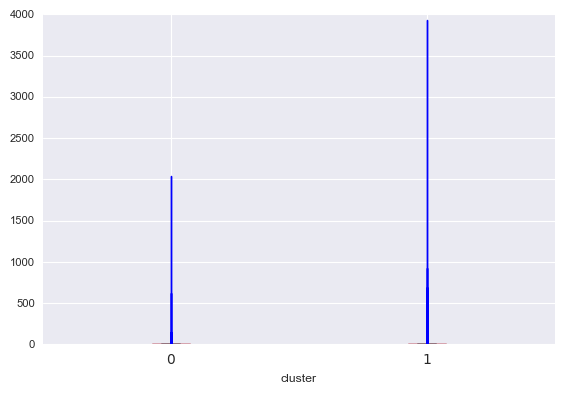
\includegraphics[width=1\textwidth]{img/collection_recovery_fee_by_cluster}}
        \end{subfigure}%
        ~ 
        \begin{subfigure}[t]{0.5\textwidth}
            \centering
            \caption{Grade }
   
            \centerline{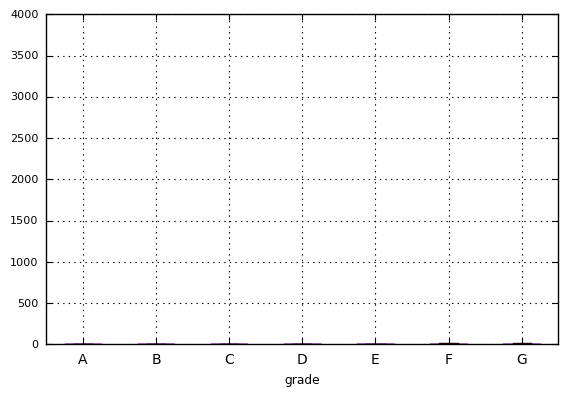
\includegraphics[width=1\textwidth]{img/collection_recovery_fee_by_grade}}

        \end{subfigure}
        \\
                \caption{funded\textunderscore amnt}
        \begin{subfigure}[t]{0.5\textwidth}
            \centering

            \centerline{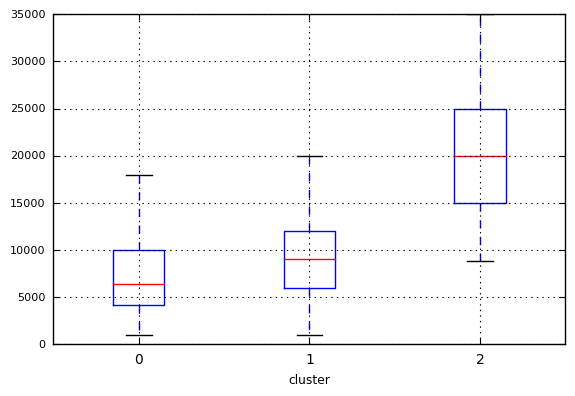
\includegraphics[width=1.05\textwidth]{img/funded_amnt_by_cluster}}
        \end{subfigure}%
        ~ 
        \begin{subfigure}[t]{0.5\textwidth}
            \centering
   
            \centerline{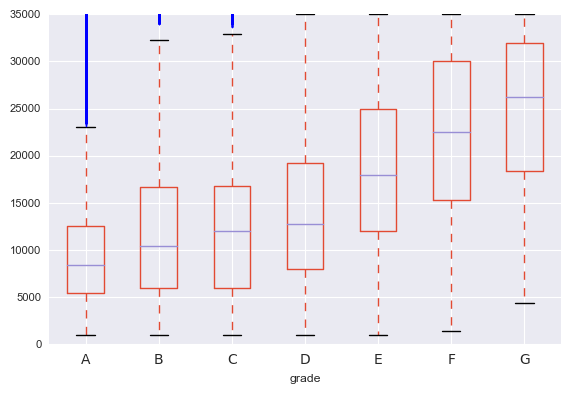
\includegraphics[width=1.05\textwidth]{img/funded_amnt_by_grade}}

        \end{subfigure}

\end{figure*}

\begin{figure*}[t!]
    \centering
        \caption{funded\textunderscore amnt\textunderscore inv }
        \begin{subfigure}[t]{0.5\textwidth}
 
            \centerline{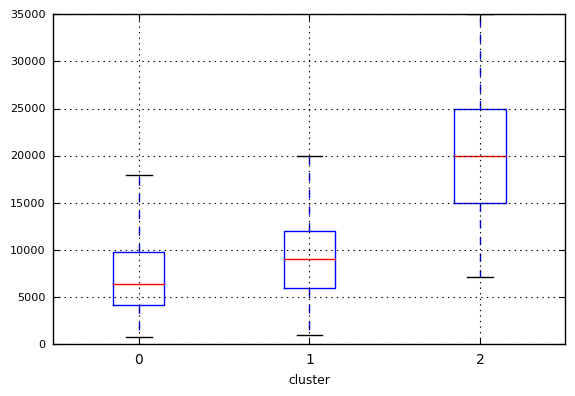
\includegraphics[width=1\textwidth]{img/funded_amnt_inv_by_cluster}}
        \end{subfigure}%
        ~ 
        \begin{subfigure}[t]{0.5\textwidth}
            \centerline{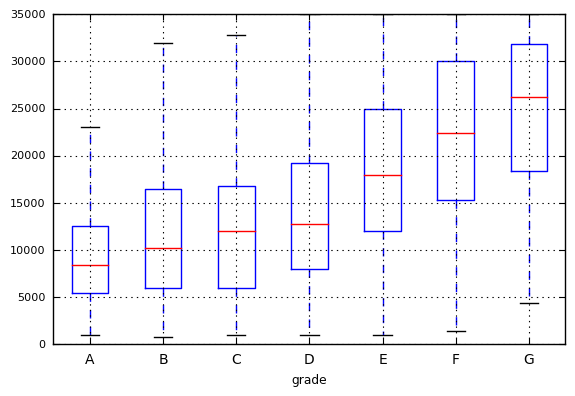
\includegraphics[width=1\textwidth]{img/funded_amnt_inv_by_grade}}

        \end{subfigure}
        \\
                \caption{installment}
        \begin{subfigure}[t]{0.5\textwidth}
            \centering

            \centerline{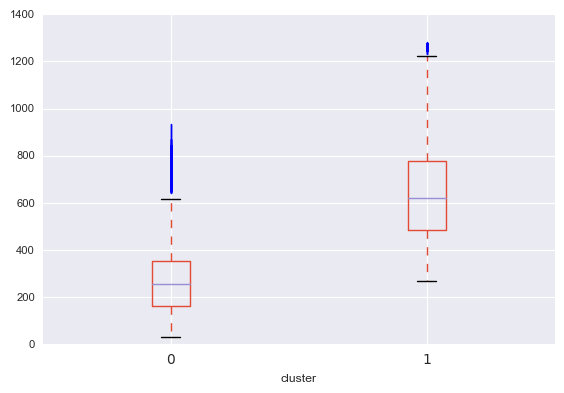
\includegraphics[width=1.05\textwidth]{img/installment_by_cluster}}
        \end{subfigure}%
        ~ 
        \begin{subfigure}[t]{0.5\textwidth}
            \centering
   
            \centerline{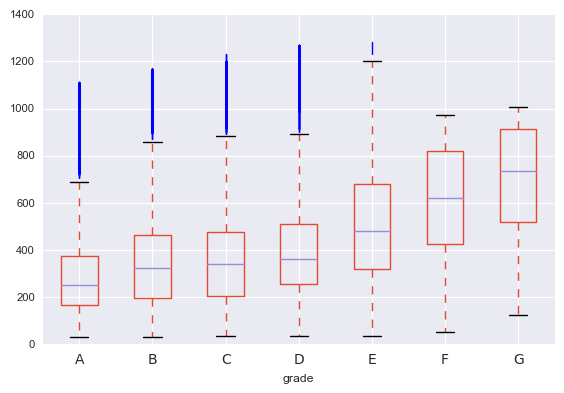
\includegraphics[width=1.05\textwidth]{img/installment_by_grade}}

        \end{subfigure}



\end{figure*}

\begin{figure*}[t!]
    \centering
        \caption{term\textunderscore float\textunderscore fee }
        \begin{subfigure}[t]{0.5\textwidth}
            \centering

            \centerline{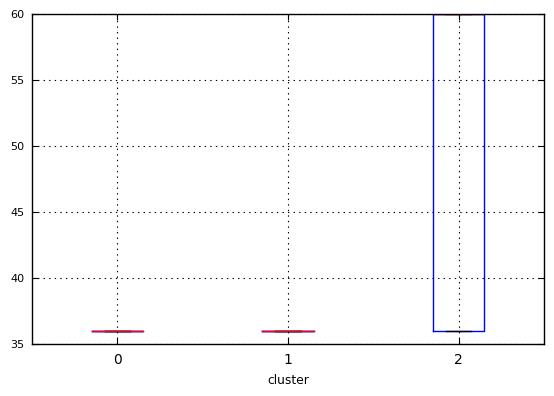
\includegraphics[width=1\textwidth]{img/term_float_by_cluster}}
        \end{subfigure}%
        ~ 
        \begin{subfigure}[t]{0.5\textwidth}
            \centering
   
            \centerline{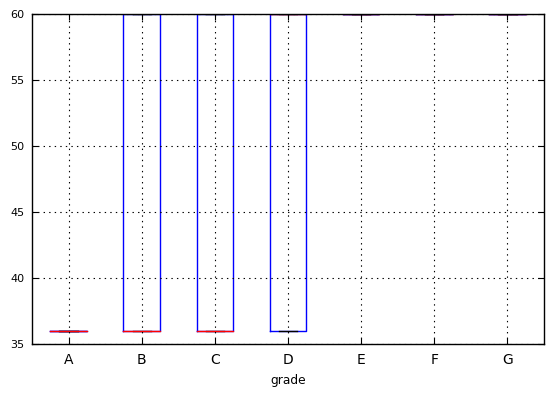
\includegraphics[width=1\textwidth]{img/term_float_by_grade}}

        \end{subfigure}
        \\
                \caption{loan\textunderscore amnt}
        \begin{subfigure}[t]{0.5\textwidth}
            \centering

            \centerline{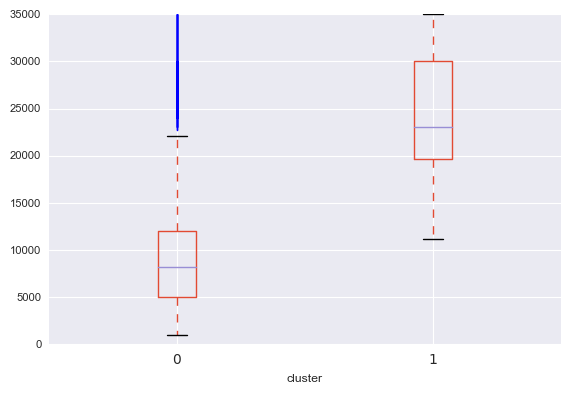
\includegraphics[width=1.05\textwidth]{img/loan_amnt_by_cluster}}
        \end{subfigure}%
        ~ 
        \begin{subfigure}[t]{0.5\textwidth}
            \centering
   
            \centerline{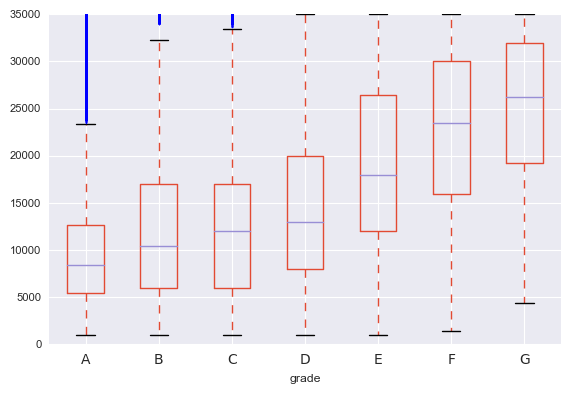
\includegraphics[width=1.05\textwidth]{img/loan_amnt_by_grade}}

        \end{subfigure}
\\
                \caption{int\textunderscore rate\textunderscore float}
        \begin{subfigure}[t]{0.5\textwidth}
            \centering

            \centerline{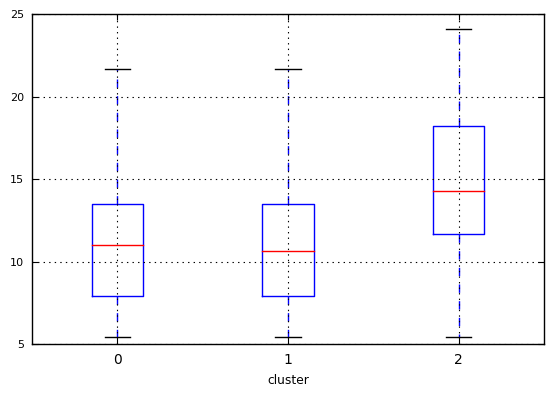
\includegraphics[width=1.05\textwidth]{img/int_rate_float_by_cluster}}
        \end{subfigure}%
        ~ 
        \begin{subfigure}[t]{0.5\textwidth}
            \centering
   
            \centerline{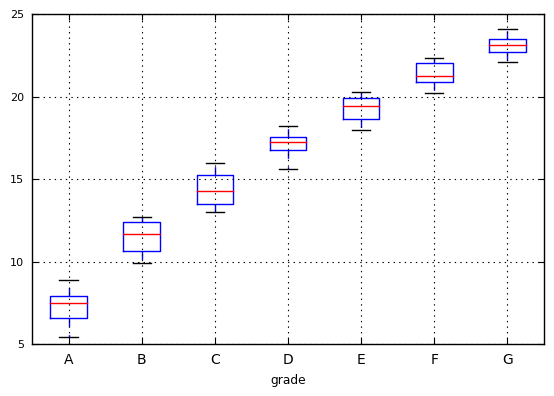
\includegraphics[width=1.05\textwidth]{img/int_rate_float_by_grade}}

        \end{subfigure}
\end{figure*}



\begin{figure*}[t!]
    \centering
        \caption{annual\textunderscore inc }
        \begin{subfigure}[t]{0.5\textwidth}
            \centering

            \centerline{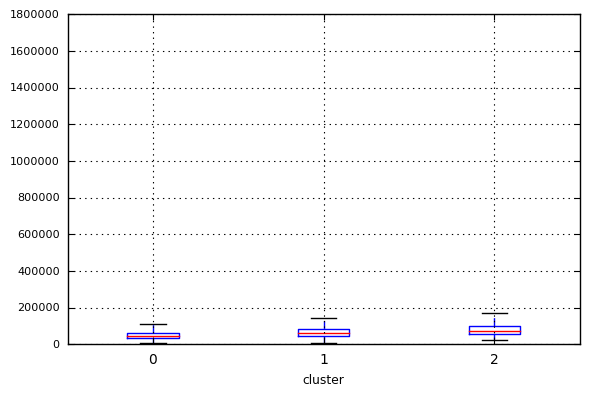
\includegraphics[width=1\textwidth]{img/annual_inc_by_cluster}}
        \end{subfigure}%
        ~ 
        \begin{subfigure}[t]{0.5\textwidth}
            \centering
   
            \centerline{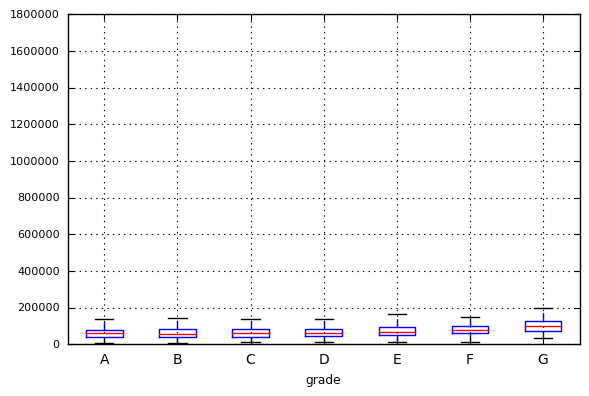
\includegraphics[width=1\textwidth]{img/annual_inc_by_grade}}

        \end{subfigure}
        \\
                \caption{delinq\textunderscore 2yrs}
        \begin{subfigure}[t]{0.5\textwidth}
            \centering

            \centerline{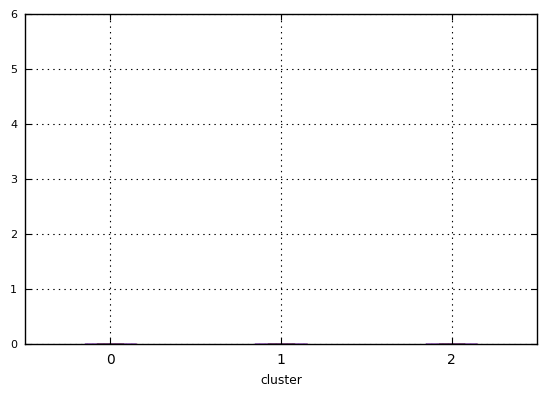
\includegraphics[width=1.05\textwidth]{img/delinq_2yrs_by_cluster}}
        \end{subfigure}%
        ~ 
        \begin{subfigure}[t]{0.5\textwidth}
            \centering
   
            \centerline{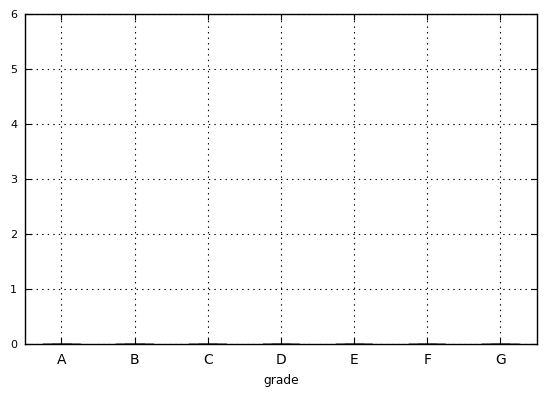
\includegraphics[width=1.05\textwidth]{img/delinq_2yrs_by_grade}}

        \end{subfigure}
\\
                \caption{recoveries}
        \begin{subfigure}[t]{0.5\textwidth}
            \centering

            \centerline{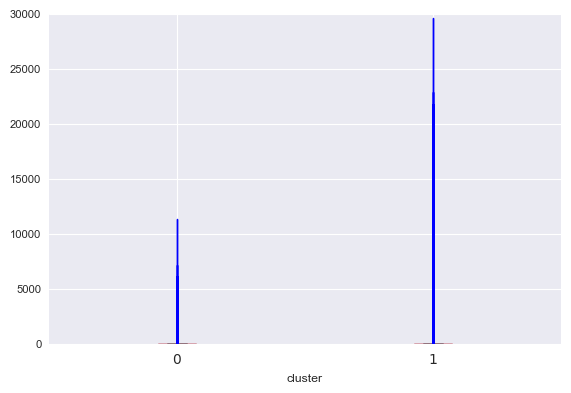
\includegraphics[width=1.05\textwidth]{img/recoveries_by_cluster}}
        \end{subfigure}%
        ~ 
        \begin{subfigure}[t]{0.5\textwidth}
            \centering
   
            \centerline{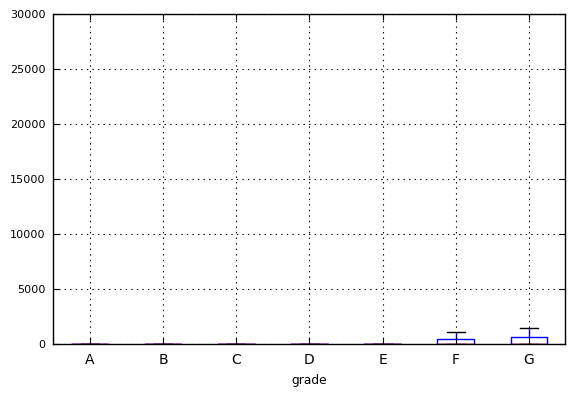
\includegraphics[width=1.05\textwidth]{img/recoveries_by_grade}}

        \end{subfigure}
\end{figure*}


\begin{figure*}[t!]
    \centering
        \caption{open\textunderscore acc }
        \begin{subfigure}[t]{0.5\textwidth}
            \centering

            \centerline{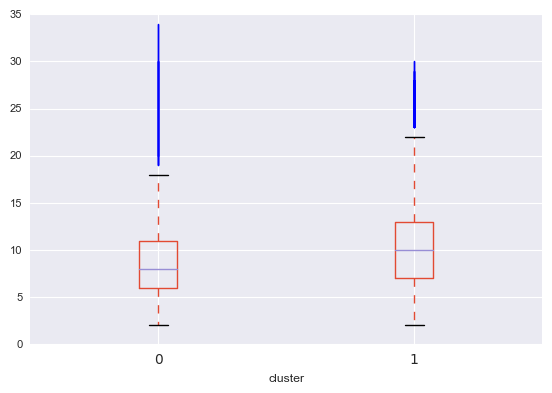
\includegraphics[width=1\textwidth]{img/open_acc_by_cluster}}
        \end{subfigure}%
        ~ 
        \begin{subfigure}[t]{0.5\textwidth}
            \centering
   
            \centerline{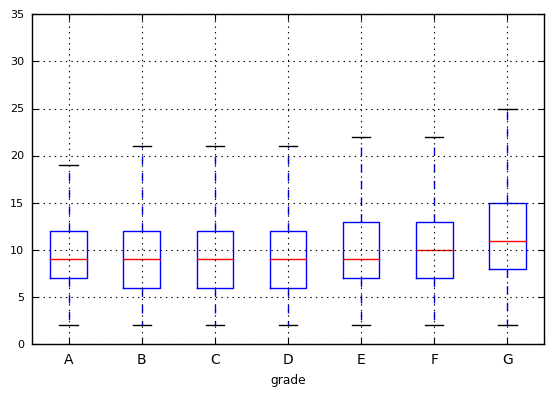
\includegraphics[width=1\textwidth]{img/open_acc_by_grade}}

        \end{subfigure}
        \\
                \caption{pub\textunderscore rec}
        \begin{subfigure}[t]{0.5\textwidth}
            \centering

            \centerline{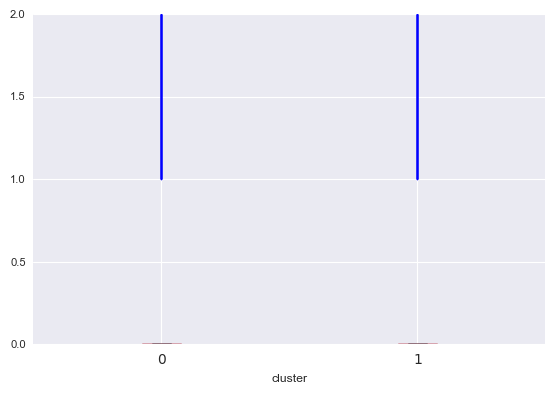
\includegraphics[width=1.05\textwidth]{img/pub_rec_by_cluster}}
        \end{subfigure}%
        ~ 
        \begin{subfigure}[t]{0.5\textwidth}
            \centering
   
            \centerline{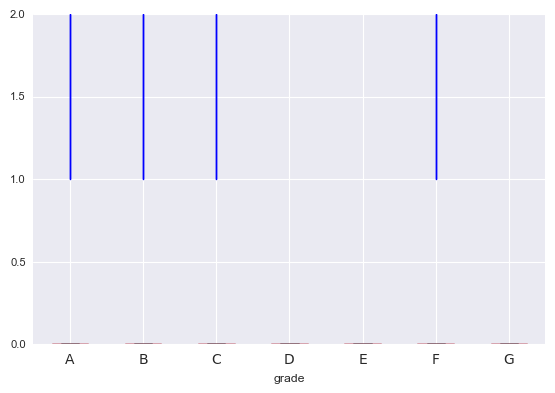
\includegraphics[width=1.05\textwidth]{img/pub_rec_by_grade}}

        \end{subfigure}
\\
                \caption{inq\textunderscore last\textunderscore 6mths}
        \begin{subfigure}[t]{0.5\textwidth}
            \centering

            \centerline{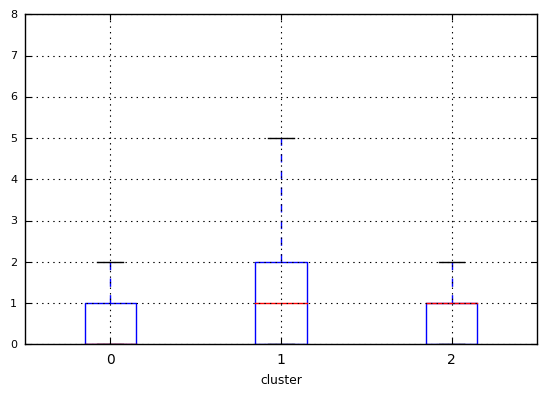
\includegraphics[width=1.05\textwidth]{img/inq_last_6mths_by_cluster}}
        \end{subfigure}%
        ~ 
        \begin{subfigure}[t]{0.5\textwidth}
            \centering
   
            \centerline{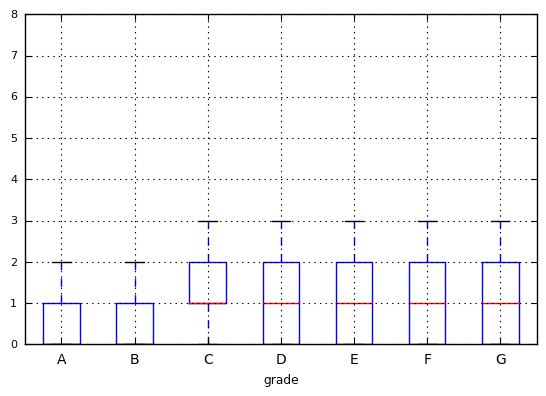
\includegraphics[width=1.05\textwidth]{img/inq_last_6mths_by_grade}}

        \end{subfigure}
\end{figure*}

\begin{figure*}[t!]
    \centering
        \caption{revol\textunderscore bal }
        \begin{subfigure}[t]{0.5\textwidth}
            \centering

            \centerline{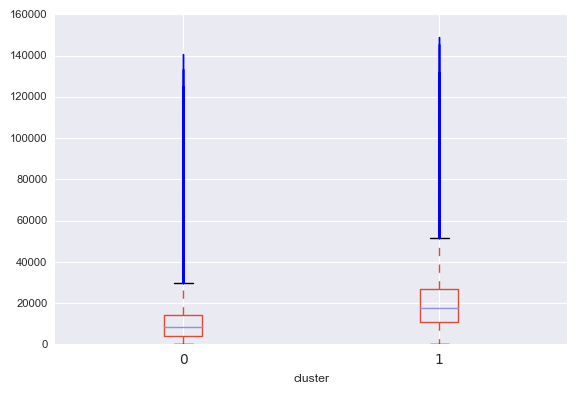
\includegraphics[width=1\textwidth]{img/revol_bal_by_cluster}}
        \end{subfigure}%
        ~ 
        \begin{subfigure}[t]{0.5\textwidth}
            \centering
   
            \centerline{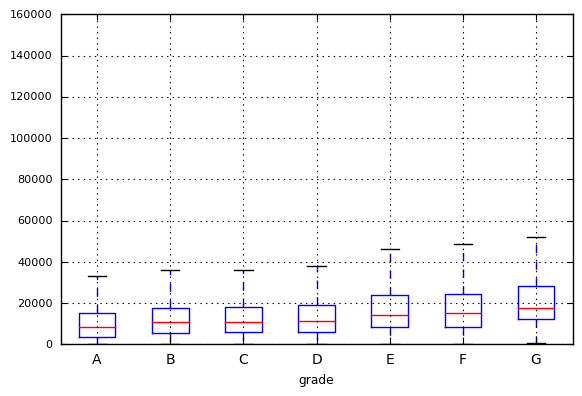
\includegraphics[width=1\textwidth]{img/revol_bal_by_grade}}

        \end{subfigure}
        \\
                \caption{total\textunderscore acc}
        \begin{subfigure}[t]{0.5\textwidth}
            \centering

            \centerline{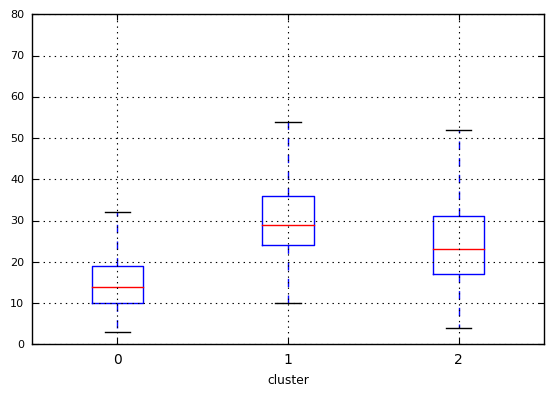
\includegraphics[width=1.05\textwidth]{img/total_acc_by_cluster}}
        \end{subfigure}%
        ~ 
        \begin{subfigure}[t]{0.5\textwidth}
            \centering
   
            \centerline{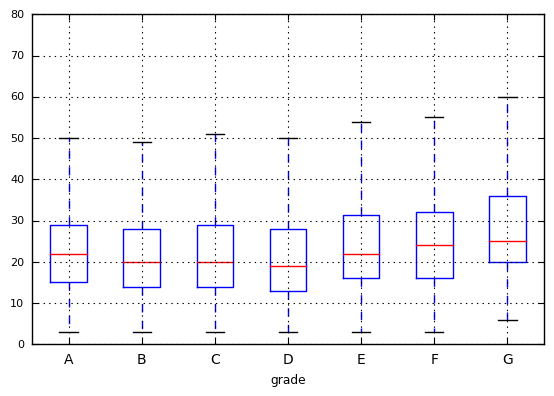
\includegraphics[width=1.05\textwidth]{img/total_acc_by_grade}}

        \end{subfigure}
\\
                \caption{out\textunderscore prncp}
        \begin{subfigure}[t]{0.5\textwidth}
            \centering

            \centerline{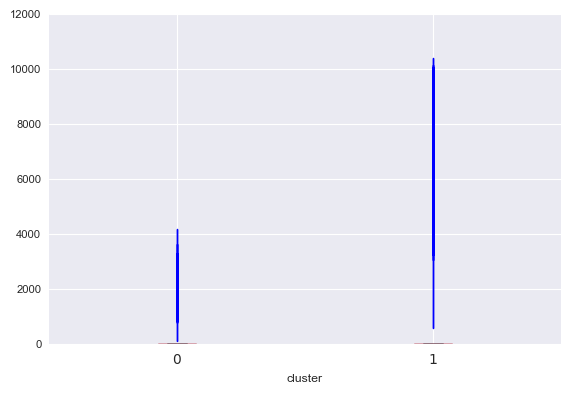
\includegraphics[width=1.05\textwidth]{img/out_prncp_by_cluster}}
        \end{subfigure}%
        ~ 
        \begin{subfigure}[t]{0.5\textwidth}
            \centering
   
            \centerline{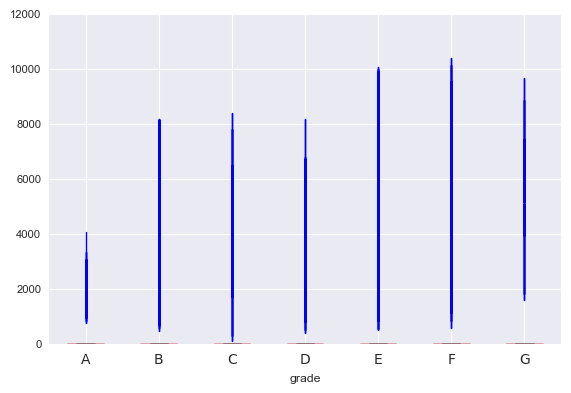
\includegraphics[width=1.05\textwidth]{img/out_prncp_by_grade}}

        \end{subfigure}
\end{figure*}


\begin{figure*}[t!]
    \centering
        \caption{total\textunderscore pymnt }
        \begin{subfigure}[t]{0.5\textwidth}
            \centering

            \centerline{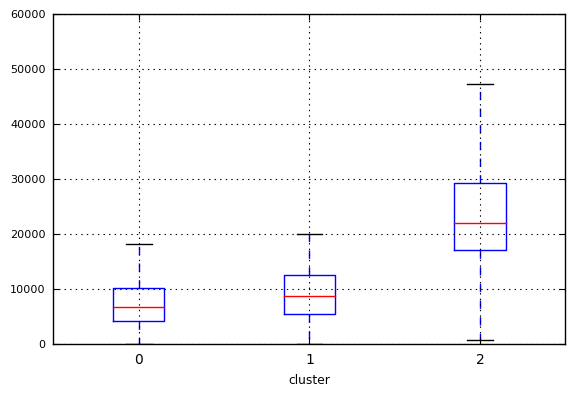
\includegraphics[width=1\textwidth]{img/total_pymnt_by_cluster}}
        \end{subfigure}%
        ~ 
        \begin{subfigure}[t]{0.5\textwidth}
            \centering
   
            \centerline{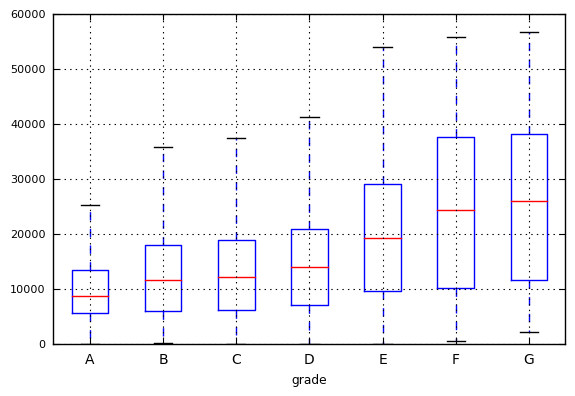
\includegraphics[width=1\textwidth]{img/total_pymnt_by_grade}}

        \end{subfigure}
        \\
                \caption{out\textunderscore prncp\textunderscore inv}
        \begin{subfigure}[t]{0.5\textwidth}
            \centering

            \centerline{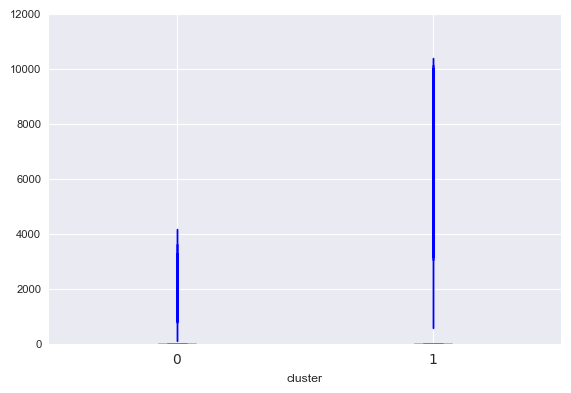
\includegraphics[width=1.05\textwidth]{img/out_prncp_inv_by_cluster}}
        \end{subfigure}%
        ~ 
        \begin{subfigure}[t]{0.5\textwidth}
            \centering
   
            \centerline{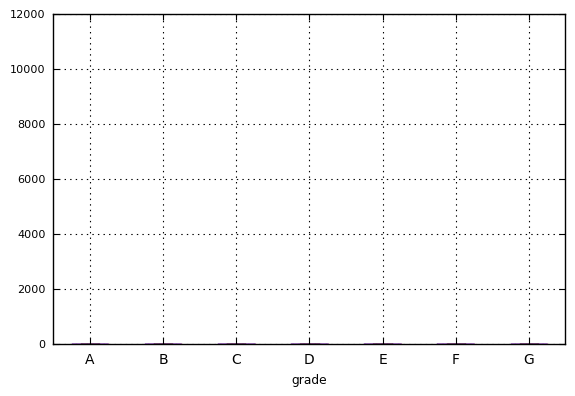
\includegraphics[width=1.05\textwidth]{img/out_prncp_inv_by_grade}}

        \end{subfigure}
\\
                \caption{total\textunderscore rec\textunderscore int }
        \begin{subfigure}[t]{0.5\textwidth}
            \centering

            \centerline{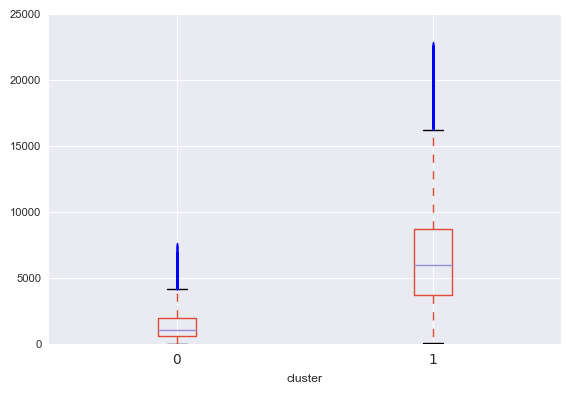
\includegraphics[width=1.05\textwidth]{img/total_rec_int_by_cluster}}
        \end{subfigure}%
        ~ 
        \begin{subfigure}[t]{0.5\textwidth}
            \centering
   
            \centerline{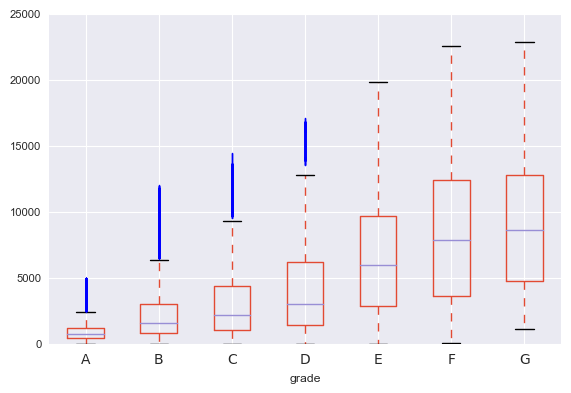
\includegraphics[width=1.05\textwidth]{img/total_rec_int_by_grade}}

        \end{subfigure}
\end{figure*}



\begin{figure*}[t!]
    \centering
        \caption{total\textunderscore pymnt\textunderscore inv }
        \begin{subfigure}[t]{0.5\textwidth}
            \centering

            \centerline{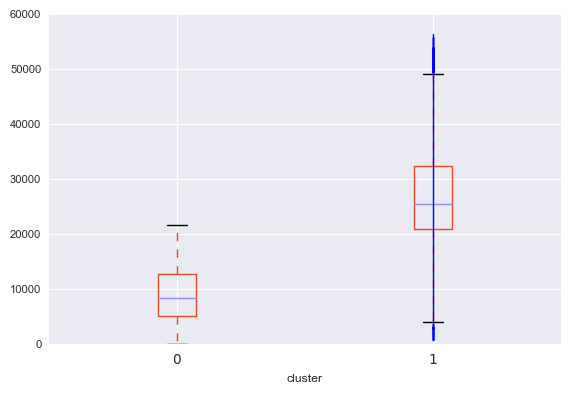
\includegraphics[width=1\textwidth]{img/total_pymnt_inv_by_cluster}}
        \end{subfigure}%
        ~ 
        \begin{subfigure}[t]{0.5\textwidth}
            \centering
   
            \centerline{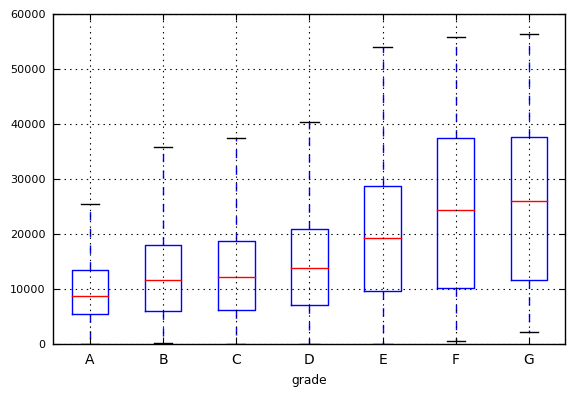
\includegraphics[width=1\textwidth]{img/total_pymnt_inv_by_grade}}

        \end{subfigure}
        \\
                \caption{last\textunderscore pymnt\textunderscore amnt}
        \begin{subfigure}[t]{0.5\textwidth}
            \centering

            \centerline{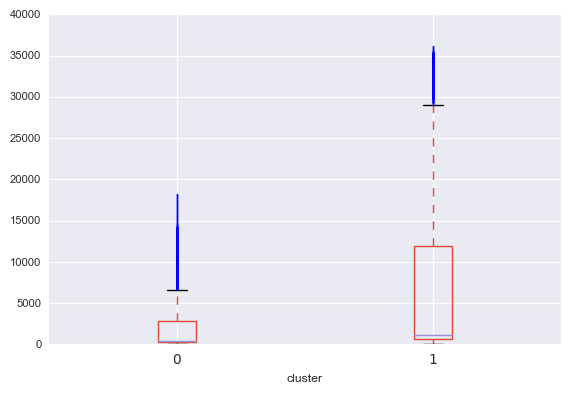
\includegraphics[width=1.05\textwidth]{img/last_pymnt_amnt_by_cluster}}
        \end{subfigure}%
        ~ 
        \begin{subfigure}[t]{0.5\textwidth}
            \centering
   
            \centerline{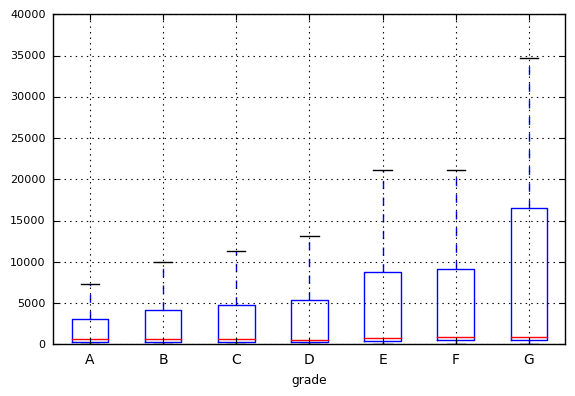
\includegraphics[width=1.05\textwidth]{img/last_pymnt_amnt_by_grade}}

        \end{subfigure}
\\
                \caption{total\textunderscore rec\textunderscore prncp }
        \begin{subfigure}[t]{0.5\textwidth}
            \centering

            \centerline{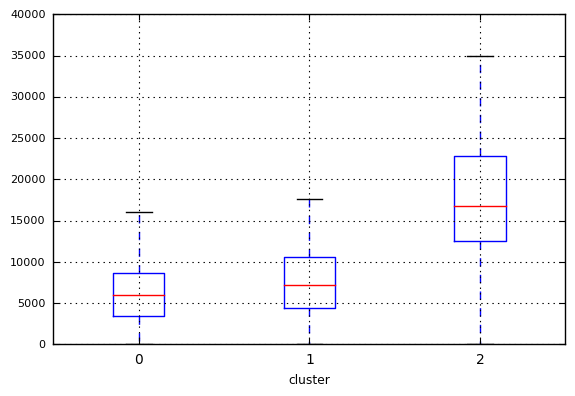
\includegraphics[width=1.05\textwidth]{img/total_rec_prncp_by_cluster}}
        \end{subfigure}%
        ~ 
        \begin{subfigure}[t]{0.5\textwidth}
            \centering
   
            \centerline{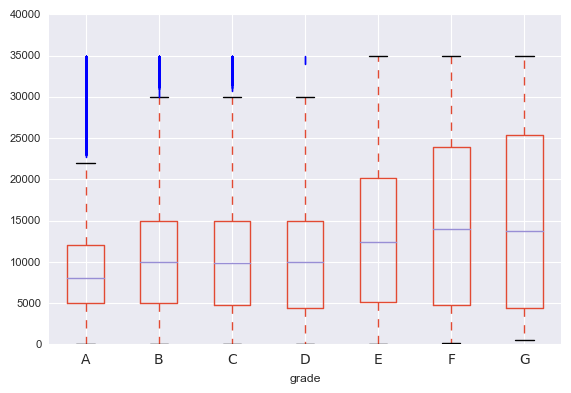
\includegraphics[width=1.05\textwidth]{img/total_rec_prncp_by_grade}}

        \end{subfigure}
\end{figure*}



\begin{figure*}[t!]
    \centering
        \caption{total\textunderscore rec\textunderscore late\textunderscore fee }
        \begin{subfigure}[t]{0.5\textwidth}
            \centering

            \centerline{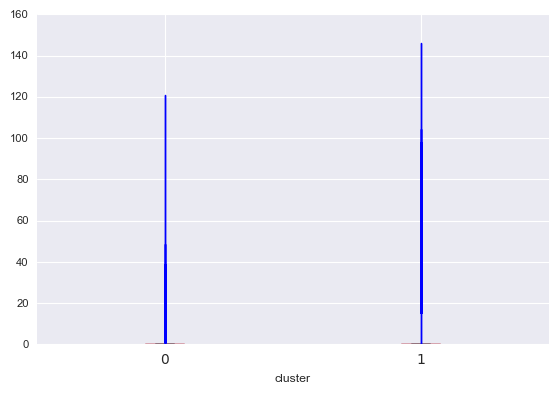
\includegraphics[width=1\textwidth]{img/total_rec_late_fee_by_cluster}}
        \end{subfigure}%
        ~ 
        \begin{subfigure}[t]{0.5\textwidth}
            \centering
   
            \centerline{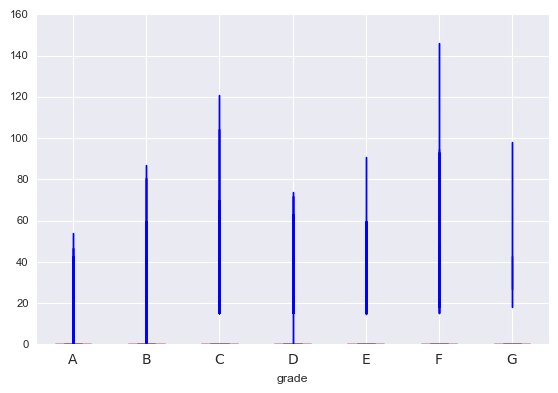
\includegraphics[width=1\textwidth]{img/total_rec_late_fee_by_grade}}

        \end{subfigure}
                \\
                \caption{dti}
        \begin{subfigure}[t]{0.5\textwidth}
            \centering

            \centerline{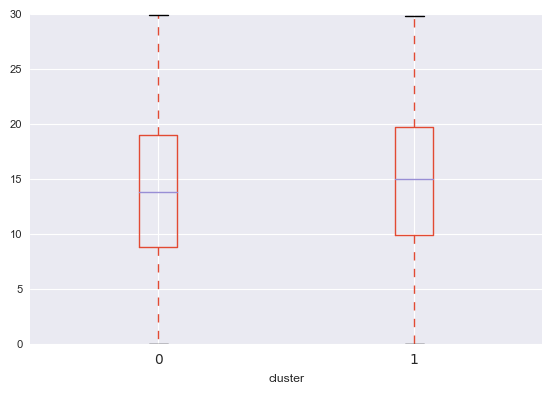
\includegraphics[width=1.05\textwidth]{img/dti_by_cluster}}
        \end{subfigure}%
        ~ 
        \begin{subfigure}[t]{0.5\textwidth}
            \centering
   
            \centerline{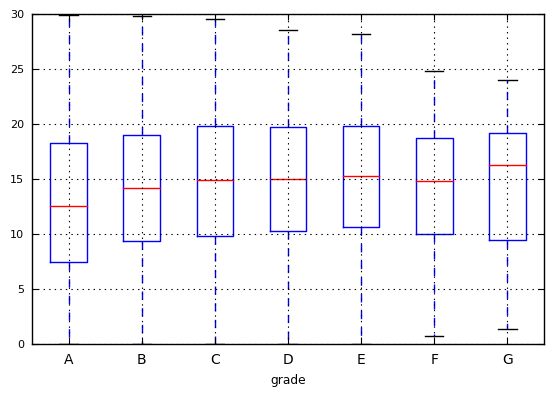
\includegraphics[width=1.05\textwidth]{img/dti_by_grade}}

        \end{subfigure}
\end{figure*}

\chapter{Correlacao entre variaveis}


\begin{landscape}

\begin{table}[]


\centering
\caption{Correlacao entre variaveis}
\label{my-label}

\scriptsize
\setlength{\tabcolsep}{1.5pt}
\begin{tabular}{lrrrrrrrrrrrrrrrrrrrrrrrrr}
    & 0      & 1      & 2      & 3      & 4      & 5      & 6      & 7      & 8      & 9      & 10     & 11     & 12     & 13     & 14     & 15     & 16     & 17     & 18     & 19     & 20     & 21     & 22     & 23     \\
0  & 1.000  & 0.999  & 0.993  & 0.487  & 0.326  & 0.956  & 0.373  & 0.033  & -0.037 & 0.025  & 0.164  & -0.065 & 0.337  & 0.259  & 0.325  & 0.325  & 0.900  & 0.899  & 0.839  & 0.738  & 0.068  & 0.169  & 0.130  & 0.440  \\
1  & 0.999  & 1.000  & 0.992  & 0.484  & 0.326  & 0.957  & 0.372  & 0.032  & -0.036 & 0.026  & 0.164  & -0.066 & 0.335  & 0.258  & 0.324  & 0.324  & 0.900  & 0.900  & 0.840  & 0.739  & 0.068  & 0.168  & 0.129  & 0.439  \\
2  & 0.993  & 0.992  & 1.000  & 0.498  & 0.333  & 0.946  & 0.373  & 0.034  & -0.036 & 0.022  & 0.165  & -0.064 & 0.338  & 0.262  & 0.328  & 0.328  & 0.893  & 0.892  & 0.831  & 0.737  & 0.068  & 0.168  & 0.129  & 0.439  \\
3  & 0.487  & 0.484  & 0.498  & 1.000  & 0.552  & 0.264  & 0.104  & 0.074  & 0.012  & 0.053  & 0.080  & -0.007 & 0.144  & 0.134  & 0.421  & 0.421  & 0.429  & 0.426  & 0.281  & 0.614  & 0.048  & 0.153  & 0.122  & 0.267  \\
4  & 0.326  & 0.326  & 0.333  & 0.552  & 1.000  & 0.291  & 0.095  & 0.098  & 0.149  & 0.188  & 0.054  & 0.082  & 0.121  & -0.002 & 0.233  & 0.233  & 0.305  & 0.305  & 0.145  & 0.554  & 0.095  & 0.154  & 0.124  & 0.168  \\
5  & 0.956  & 0.957  & 0.946  & 0.264  & 0.291  & 1.000  & 0.387  & 0.022  & -0.027 & 0.030  & 0.164  & -0.060 & 0.334  & 0.241  & 0.219  & 0.219  & 0.866  & 0.867  & 0.836  & 0.648  & 0.072  & 0.144  & 0.110  & 0.399  \\
6  & 0.373  & 0.372  & 0.373  & 0.104  & 0.095  & 0.387  & 1.000  & -0.185 & 0.035  & 0.046  & 0.199  & -0.029 & 0.367  & 0.310  & 0.094  & 0.094  & 0.367  & 0.367  & 0.365  & 0.259  & 0.034  & 0.029  & 0.032  & 0.200  \\
7  & 0.033  & 0.032  & 0.034  & 0.074  & 0.098  & 0.022  & -0.185 & 1.000  & -0.049 & 0.023  & 0.280  & -0.017 & 0.221  & 0.224  & 0.049  & 0.049  & 0.029  & 0.029  & -0.001 & 0.083  & 0.005  & 0.032  & 0.030  & -0.015 \\
8  & -0.037 & -0.036 & -0.036 & 0.012  & 0.149  & -0.027 & 0.035  & -0.049 & 1.000  & -0.006 & 0.007  & 0.003  & -0.066 & 0.069  & 0.014  & 0.014  & -0.026 & -0.026 & -0.048 & 0.031  & 0.036  & 0.012  & 0.015  & -0.010 \\
9  & 0.025  & 0.026  & 0.022  & 0.053  & 0.188  & 0.030  & 0.046  & 0.023  & -0.006 & 1.000  & 0.097  & 0.030  & -0.018 & 0.116  & -0.016 & -0.015 & 0.014  & 0.016  & -0.002 & 0.042  & 0.013  & 0.022  & 0.029  & 0.057  \\
10 & 0.164  & 0.164  & 0.165  & 0.080  & 0.054  & 0.164  & 0.199  & 0.280  & 0.007  & 0.097  & 1.000  & -0.006 & 0.279  & 0.674  & 0.046  & 0.046  & 0.158  & 0.158  & 0.149  & 0.126  & 0.008  & 0.038  & 0.031  & 0.080  \\
11 & -0.065 & -0.066 & -0.064 & -0.007 & 0.082  & -0.060 & -0.029 & -0.017 & 0.003  & 0.030  & -0.006 & 1.000  & -0.077 & -0.027 & -0.023 & -0.023 & -0.060 & -0.061 & -0.069 & -0.018 & -0.009 & -0.011 & -0.014 & -0.023 \\
12 & 0.337  & 0.335  & 0.338  & 0.144  & 0.121  & 0.334  & 0.367  & 0.221  & -0.066 & -0.018 & 0.279  & -0.077 & 1.000  & 0.314  & 0.130  & 0.130  & 0.326  & 0.325  & 0.302  & 0.272  & 0.016  & 0.059  & 0.053  & 0.140  \\
13 & 0.259  & 0.258  & 0.262  & 0.134  & -0.002 & 0.241  & 0.310  & 0.224  & 0.069  & 0.116  & 0.674  & -0.027 & 0.314  & 1.000  & 0.062  & 0.062  & 0.237  & 0.237  & 0.236  & 0.160  & -0.005 & 0.045  & 0.047  & 0.164  \\
14 & 0.325  & 0.324  & 0.328  & 0.421  & 0.233  & 0.219  & 0.094  & 0.049  & 0.014  & -0.016 & 0.046  & -0.023 & 0.130  & 0.062  & 1.000  & 1.000  & 0.363  & 0.361  & 0.218  & 0.612  & 0.036  & -0.047 & -0.034 & -0.153 \\
15 & 0.325  & 0.324  & 0.328  & 0.421  & 0.233  & 0.219  & 0.094  & 0.049  & 0.014  & -0.015 & 0.046  & -0.023 & 0.130  & 0.062  & 1.000  & 1.000  & 0.363  & 0.361  & 0.218  & 0.612  & 0.036  & -0.047 & -0.034 & -0.153 \\
16 & 0.900  & 0.900  & 0.893  & 0.429  & 0.305  & 0.866  & 0.367  & 0.029  & -0.026 & 0.014  & 0.158  & -0.060 & 0.326  & 0.237  & 0.363  & 0.363  & 1.000  & 1.000  & 0.957  & 0.803  & 0.029  & 0.030  & 0.038  & 0.504  \\
17 & 0.899  & 0.900  & 0.892  & 0.426  & 0.305  & 0.867  & 0.367  & 0.029  & -0.026 & 0.016  & 0.158  & -0.061 & 0.325  & 0.237  & 0.361  & 0.361  & 1.000  & 1.000  & 0.958  & 0.802  & 0.029  & 0.029  & 0.037  & 0.503  \\
18 & 0.839  & 0.840  & 0.831  & 0.281  & 0.145  & 0.836  & 0.365  & -0.001 & -0.048 & -0.002 & 0.149  & -0.069 & 0.302  & 0.236  & 0.218  & 0.218  & 0.957  & 0.958  & 1.000  & 0.611  & -0.016 & -0.113 & -0.078 & 0.594  \\
19 & 0.738  & 0.739  & 0.737  & 0.614  & 0.554  & 0.648  & 0.259  & 0.083  & 0.031  & 0.042  & 0.126  & -0.018 & 0.272  & 0.160  & 0.612  & 0.612  & 0.803  & 0.802  & 0.611  & 1.000  & 0.108  & 0.096  & 0.088  & 0.168  \\
20 & 0.068  & 0.068  & 0.068  & 0.048  & 0.095  & 0.072  & 0.034  & 0.005  & 0.036  & 0.013  & 0.008  & -0.009 & 0.016  & -0.005 & 0.036  & 0.036  & 0.029  & 0.029  & -0.016 & 0.108  & 1.000  & 0.065  & 0.058  & -0.067 \\
21 & 0.169  & 0.168  & 0.168  & 0.153  & 0.154  & 0.144  & 0.029  & 0.032  & 0.012  & 0.022  & 0.038  & -0.011 & 0.059  & 0.045  & -0.047 & -0.047 & 0.030  & 0.029  & -0.113 & 0.096  & 0.065  & 1.000  & 0.797  & -0.083 \\
22 & 0.130  & 0.129  & 0.129  & 0.122  & 0.124  & 0.110  & 0.032  & 0.030  & 0.015  & 0.029  & 0.031  & -0.014 & 0.053  & 0.047  & -0.034 & -0.034 & 0.038  & 0.037  & -0.078 & 0.088  & 0.058  & 0.797  & 1.000  & -0.060 \\
23 & 0.440  & 0.439  & 0.439  & 0.267  & 0.168  & 0.399  & 0.200  & -0.015 & -0.010 & 0.057  & 0.080  & -0.023 & 0.140  & 0.164  & -0.153 & -0.153 & 0.504  & 0.503  & 0.594  & 0.168  & -0.067 & -0.083 & -0.060 & 1.000 
\end{tabular}
\end{table}

\end{landscape}



% ---
%\chapter{Morbi ultrices rutrum lorem.}
% ---
%\lipsum[30]

% ---
%\chapter{Cras non urna sed feugiat cum sociis natoque penatibus et magnis dis
%parturient montes nascetur ridiculus mus}
% ---

%\lipsum[31]

% ---
%\chapter{Fusce facilisis lacinia dui}
% ---

%\lipsum[32]

\end{anexosenv}